\section{Grundlagen des Cloud Computing}
\label{sec:cloud-computing}

Im folgenden Kapitel werden die Grundlagen und eine Definition des Cloud Computing erarbeitet. Hierbei werden die grundlegenden Konzepte, Bereitstellungsmodelle und Abstraktionsebenen des Cloud Computing erläutert.

\subsection{Was ist Cloud Computing}
Das \ac{NIST}, auf dessen Definition sich in der Literatur häufig bezogen wird \cite[Vgl.][S. 4f]{Reinheimer2018}, definiert Cloud Computing wie folgt:
%Cloud Computing ist ein Modell der Bereitstellung von Computing Ressourcen (z. B. Netzwerke, Server, Speicher, Anwendungen und Services). Diese werden über das Netzwerk zu Verfügung gestellt um mit geringem Managementaufwand schnell freigegeben und bereitgestellt werden können

\textit{''Cloud computing is a model for enabling ubiquitous, convenient, on-demand network access to a shared pool of configurable computing resources (e.g., networks, servers, storage, applications, and services) that can be rapidly provisioned and released with minimal management effort or service provider interaction. This cloud model is composed of five essential characteristics, three service models, and four deployment models.''} \cite[][S. 2]{Mell2011}

Demnach wird Cloud Computing als Modell der Bereitstellung von Computing Ressourcen, wie zum Beispiel Server, Anwendungen oder Speicher definiert, die über das Netzwerk zu Verfügung gestellt werden \cite[Vgl.][S. 5]{Reinheimer2018}.

Nach Hentschel und Leyh (2018), Zhao (2014), Maenhaut (2016) und Surianarayanan (2019) kann man Cloud Services grundsätzlich in drei Abstraktionsebenen einteilen. Diese sind \textbf{\ac{SaaS}}, \textbf{\ac{PaaS}} und \textbf{\ac{IaaS}}, welche auch zu \ac{XaaS} zusammengefasst werden \cite[Vgl.][S. 9]{Reinheimer2018}\cite[Vgl.][S. 143f]{Zhao2014}\cite[Vgl.][S. 32ff]{Maenhaut2016}\cite[Vgl.][S. 226ff]{Surianarayanan2019}.
% Darüber hinaus haben sich jedoch noch einige weitere Bereitstellungsmodelle entwickelt, die überwiegend als ''Unterkategorien'' von \ac{PaaS} einzuordnen sind. Dazu gehören unter anderem \ac{CaaS} \cite[Vgl.][]{Luber2019}, \ac{BaaS} und \ac{FaaS} \cite[Vgl.][]{Luber2022}.
Darüber hinaus kann noch das \textit{Serverless Computing} als relativ neuer Trend und weitere Ausprägung des \ac{PaaS} Modells verstanden werden \cite[Vgl.][S. 11ff]{CNCF2018} \pagebreak

Die in Abbildung \ref{fig:XaaS} dargestellte unterste der drei genannten Abstraktionsschichten ist \ac{IaaS}, welche Infrastruktur, wie zum Beispiel Netzwerk, Server oder Speicher, bereitstellt. Ein Beispiel für einen \ac{IaaS} Service ist das deutsche Unternehmen \textit{Profitbricks}, welches Rechenleistung und Speicherkapazität in einem Virtuellen Rechenzentrum bereitstellt, die zu Virtuellen Servern konfiguriert werden können \cite[Vgl.][S. 12]{Reinheimer2018}.

\begin{figure}[H]
    \centering
    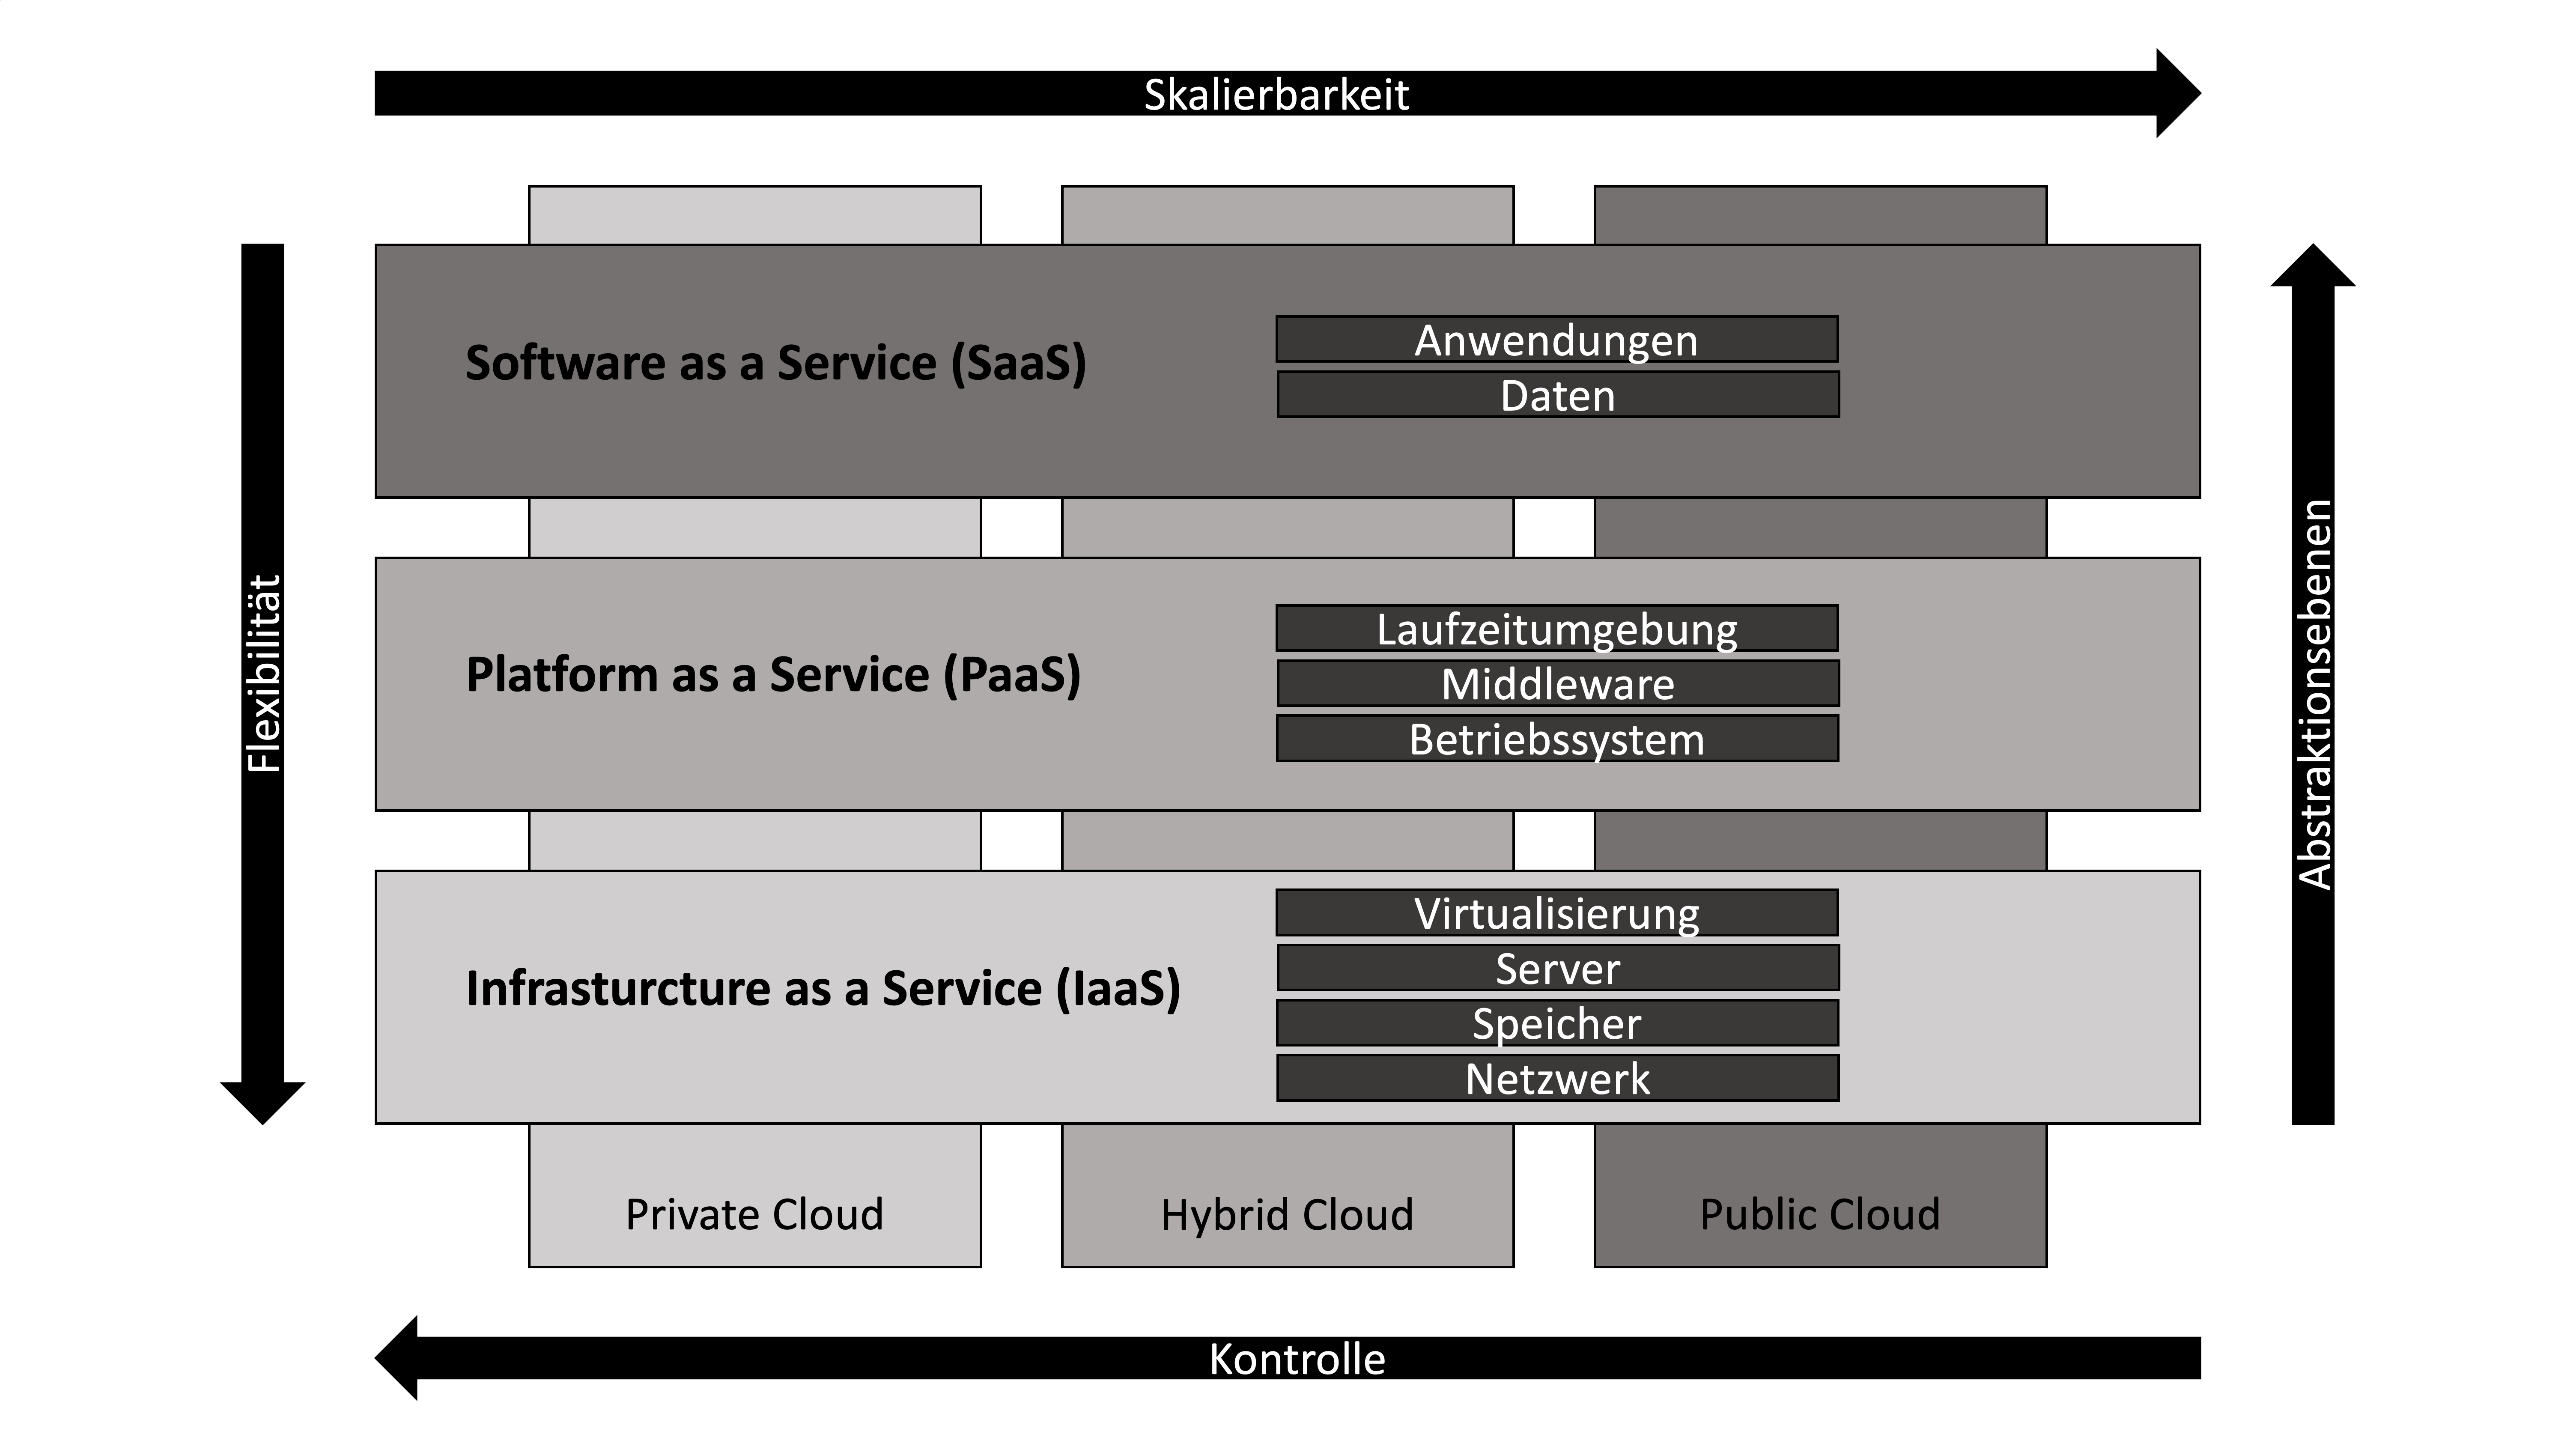
\includegraphics[height=0.5\textwidth]{xaas.png}
    \caption{Eine Übersicht der Cloud Service Modelle \cite[Eigene Darstellung nach][S. 33]{Maenhaut2016}\cite[Ergänzt durch][]{Toroman2018}}
    \label{fig:XaaS}
\end{figure}

Diese Infrastruktur kann sowohl physisch als auch virtuell zur Verfügung gestellt werden \cite[Vgl.][S. 9f]{Reinheimer2018}. Die darüber liegend dargestellte Schicht ist \ac{PaaS}, welche die darunterliegende Infrastrukturebene abstrahiert und als Basis zur Anwendungsentwicklung genutzt werden kann, indem zum Beispiel bereits ein Betriebssystem, Middleware und eine Laufzeitumgebung bereitgestellt werden \cite[Vgl.][S. 10]{Reinheimer2018}. Anbieter für \ac{PaaS} Plattformen sind unter anderem Google (Google App Engine) und \textit{Jelastic} mit einer Plattform zur Entwicklung von Webanwendungen in verschiedenen Entwicklungsumgebungen \cite[Vgl.][S. 13]{Reinheimer2018}. Die oberste Abstraktionsebene ist \ac{SaaS}, welche standardisierte Anwendungen zur Verfügung stellt und somit ohne Verwaltung der zugrundeliegenden Ressourcen und Bereitstellung der Anwendungen genutzt werden kann. Die Bereitstellung der Anwendung wird vom Provider übernommen \cite[Vgl.][S. 11]{Reinheimer2018}. Als Beispiel für \ac{SaaS} wird von Hentschel und Leyh SAP S/4Hana herangezogen. Die Software wird in SAP eigenen Rechenzentren bereitgestellt und auch Support und Wartung vollständig von SAP übernommen. Anwender können sich vollständig auf die Nutzung der Software konzentrieren \cite[Vgl.][S. 14]{Reinheimer2018}. \pagebreak

Generell wird die Cloud darüber hinaus, wie in Abbildung \ref{fig:XaaS} bereits angedeutet, in drei Organisationsdimensionen eingeteilt \cite[Vgl. auch im Folgenden][S. 7ff]{Reinheimer2018}:
\begin{itemize}
\item \textbf{Private Cloud:} Die Private Cloud bietet die exklusive Nutzung durch eine Organisation. Die IT-Infrastruktur einer Private Cloud kann entweder im Unternehmenseigenen Rechenzentrum untergebracht oder auch von Dienstleistern bereitgestellt werden.
\item \textbf{Public Cloud:} In der Public Cloud ist die Infrastruktur für mehr Anwender zugänglich und muss geteilt werden. Dafür muss als Anwender oft auch nur für die tatsächlich genutzte Leistung gezahlt werden. Da die Infrastruktur jedoch gleichzeitig von vielen genutzt wird, ist zum Beispiel der Betrieb von sicherheitskritischen Anwendungen schwierig.
\item \textbf{Hybrid Cloud:} Die Hybrid Cloud bildet eine kombinierte Anwendung aus der Public Cloud und der Private Cloud. Diese bietet dem Anwender die Möglichkeit gewisse Anwendungen in die Public Cloud auszulagern, ohne die Vorteile der Private Cloud für sicherheitsrelevante Anwendungen aufgeben zu müssen. Als weiterer möglicher Aspekt kann bei einem Hybrid Cloud Modell die Rechenleistung der Private Cloud bei Spitzenlast durch die Public Cloud für nicht sicherheitskritische Anwendungen erweitert werden. 
\end{itemize} \pagebreak

\subsection{Entwicklung des Cloud Computing}
\label{sec:entwicklung}
Die Entwicklung des Cloud Computing und dessen Vorgängerkonzepte ist bis in die 90er Jahre zurückzuführen. Ein von Hentschel und Leyh (2018) hervorgehobener Vorgänger bildet das Grid Computing. Damit war bereits eine dezentrale Ressourcenkontrolle mir standardisierten Protokollen und Schnittstellen realisiert. Das Cloud Computing bietet vergleichbare Eigenschaften, jedoch rückt der Fokus hier auf wirtschaftliche Kriterien und die Zentralisierung von Ressourcen in Rechenzentren \cite[Vgl.][S. 5f]{Reinheimer2018}.

Salesforce war eines der ersten Unternehmen, welches 1999 Anwendungen über eine Webseite bereitgestellt hat, gefolgt von \ac{AWS} in 2002, welche Speicher und Rechenleistung als Services bereitstellten \cite[Vgl.][S. 17f]{Srivastava2018}.

\begin{figure}[H]
    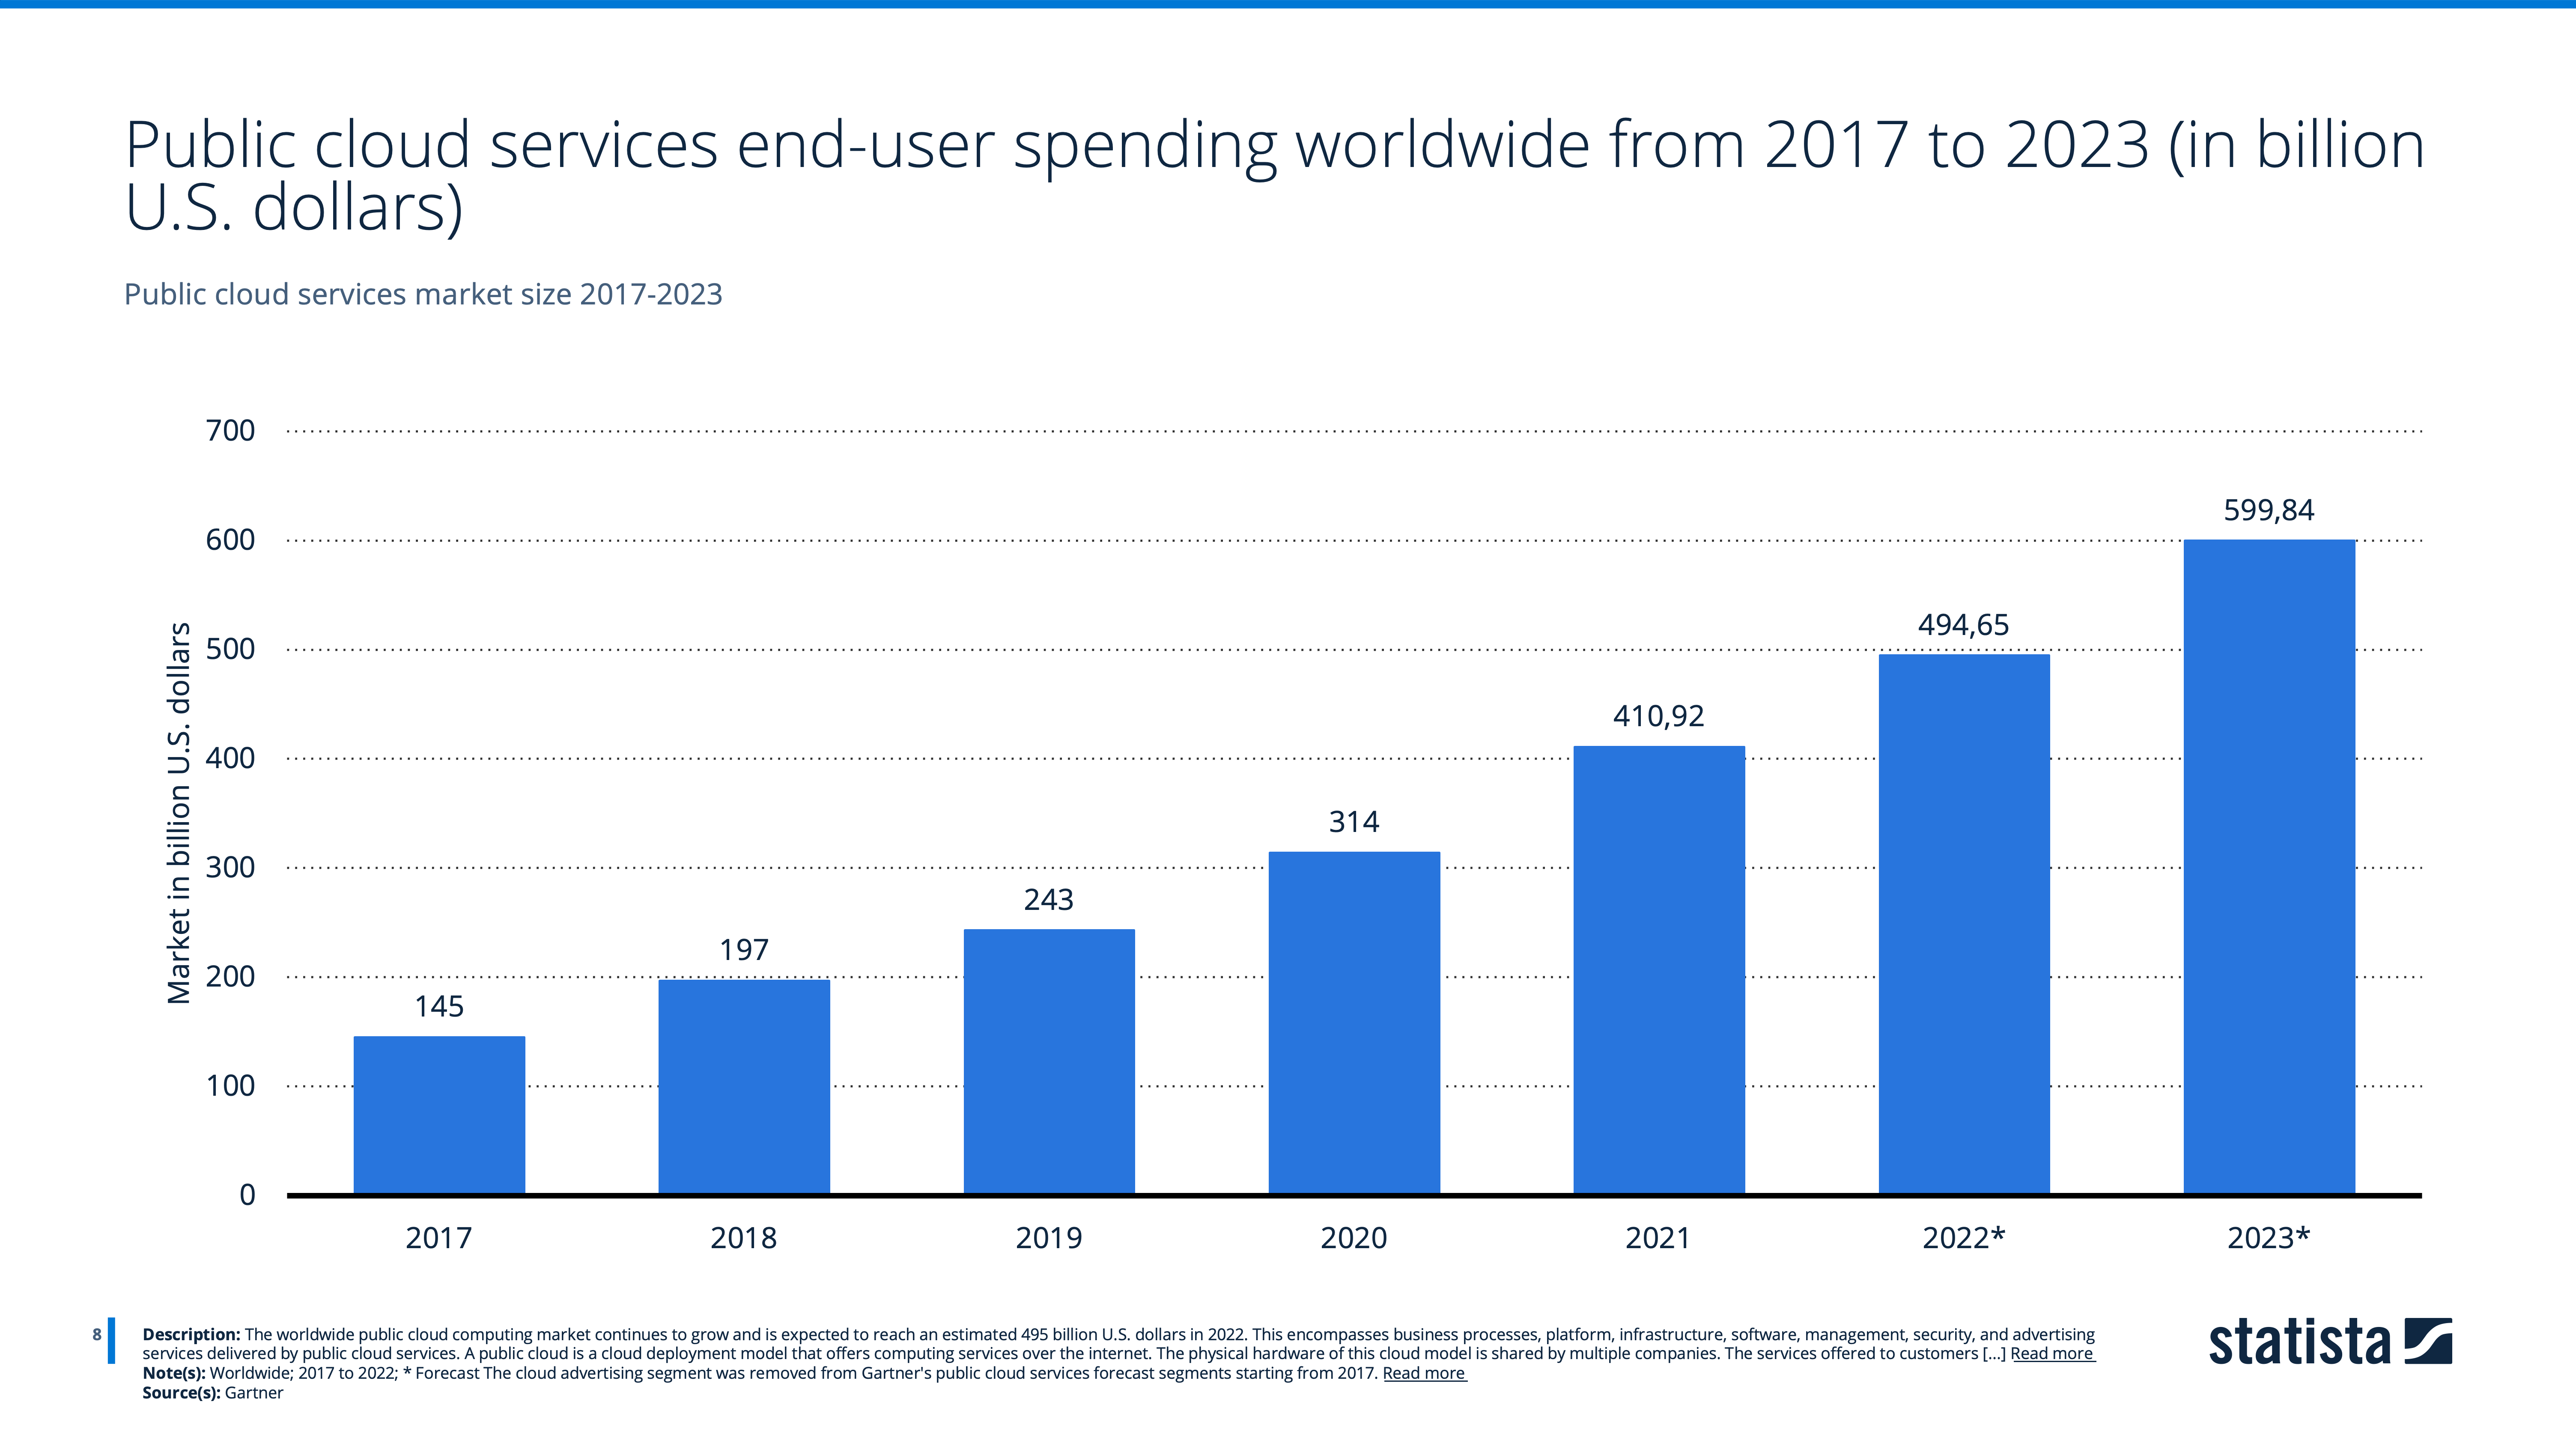
\includegraphics[width=\textwidth]{public_cloud_spending.png}
    \caption{Die Verkaufsleistungen der Public Cloud in den letzten Jahren \cite[S. 8]{Statista2022}}
    \label{fig:public_cloud_spending}
\end{figure}

Aus einem Dossier von Statista 2022 geht in der in Abbildung \ref{fig:public_cloud_spending} gezeigten Statistik hervor, dass sich die Ausgaben für Public Cloud Services von 2017 bis 2023 voraussichtlich mehr als vervierfachen werden \cite[Vgl.][S. 8]{Statista2022}. Auch weitere Statistiken desselben Dossiers machen einen stetig steigende Entwicklung hinsichtlich des Cloud Computing deutlich \cite[Vgl. unter anderem][S. 11ff]{Statista2022}. \pagebreak

Abbildung \ref{fig:it-spending} zeigt darüber hinaus, wie sich die IT-Ausgaben in Unternehmen weltweit in den letzten Jahren immer stärker auf Cloud Infrastruktur fokussiert haben und sich von traditioneller IT-Infrastruktur zurückziehen.

\begin{figure}[H]
    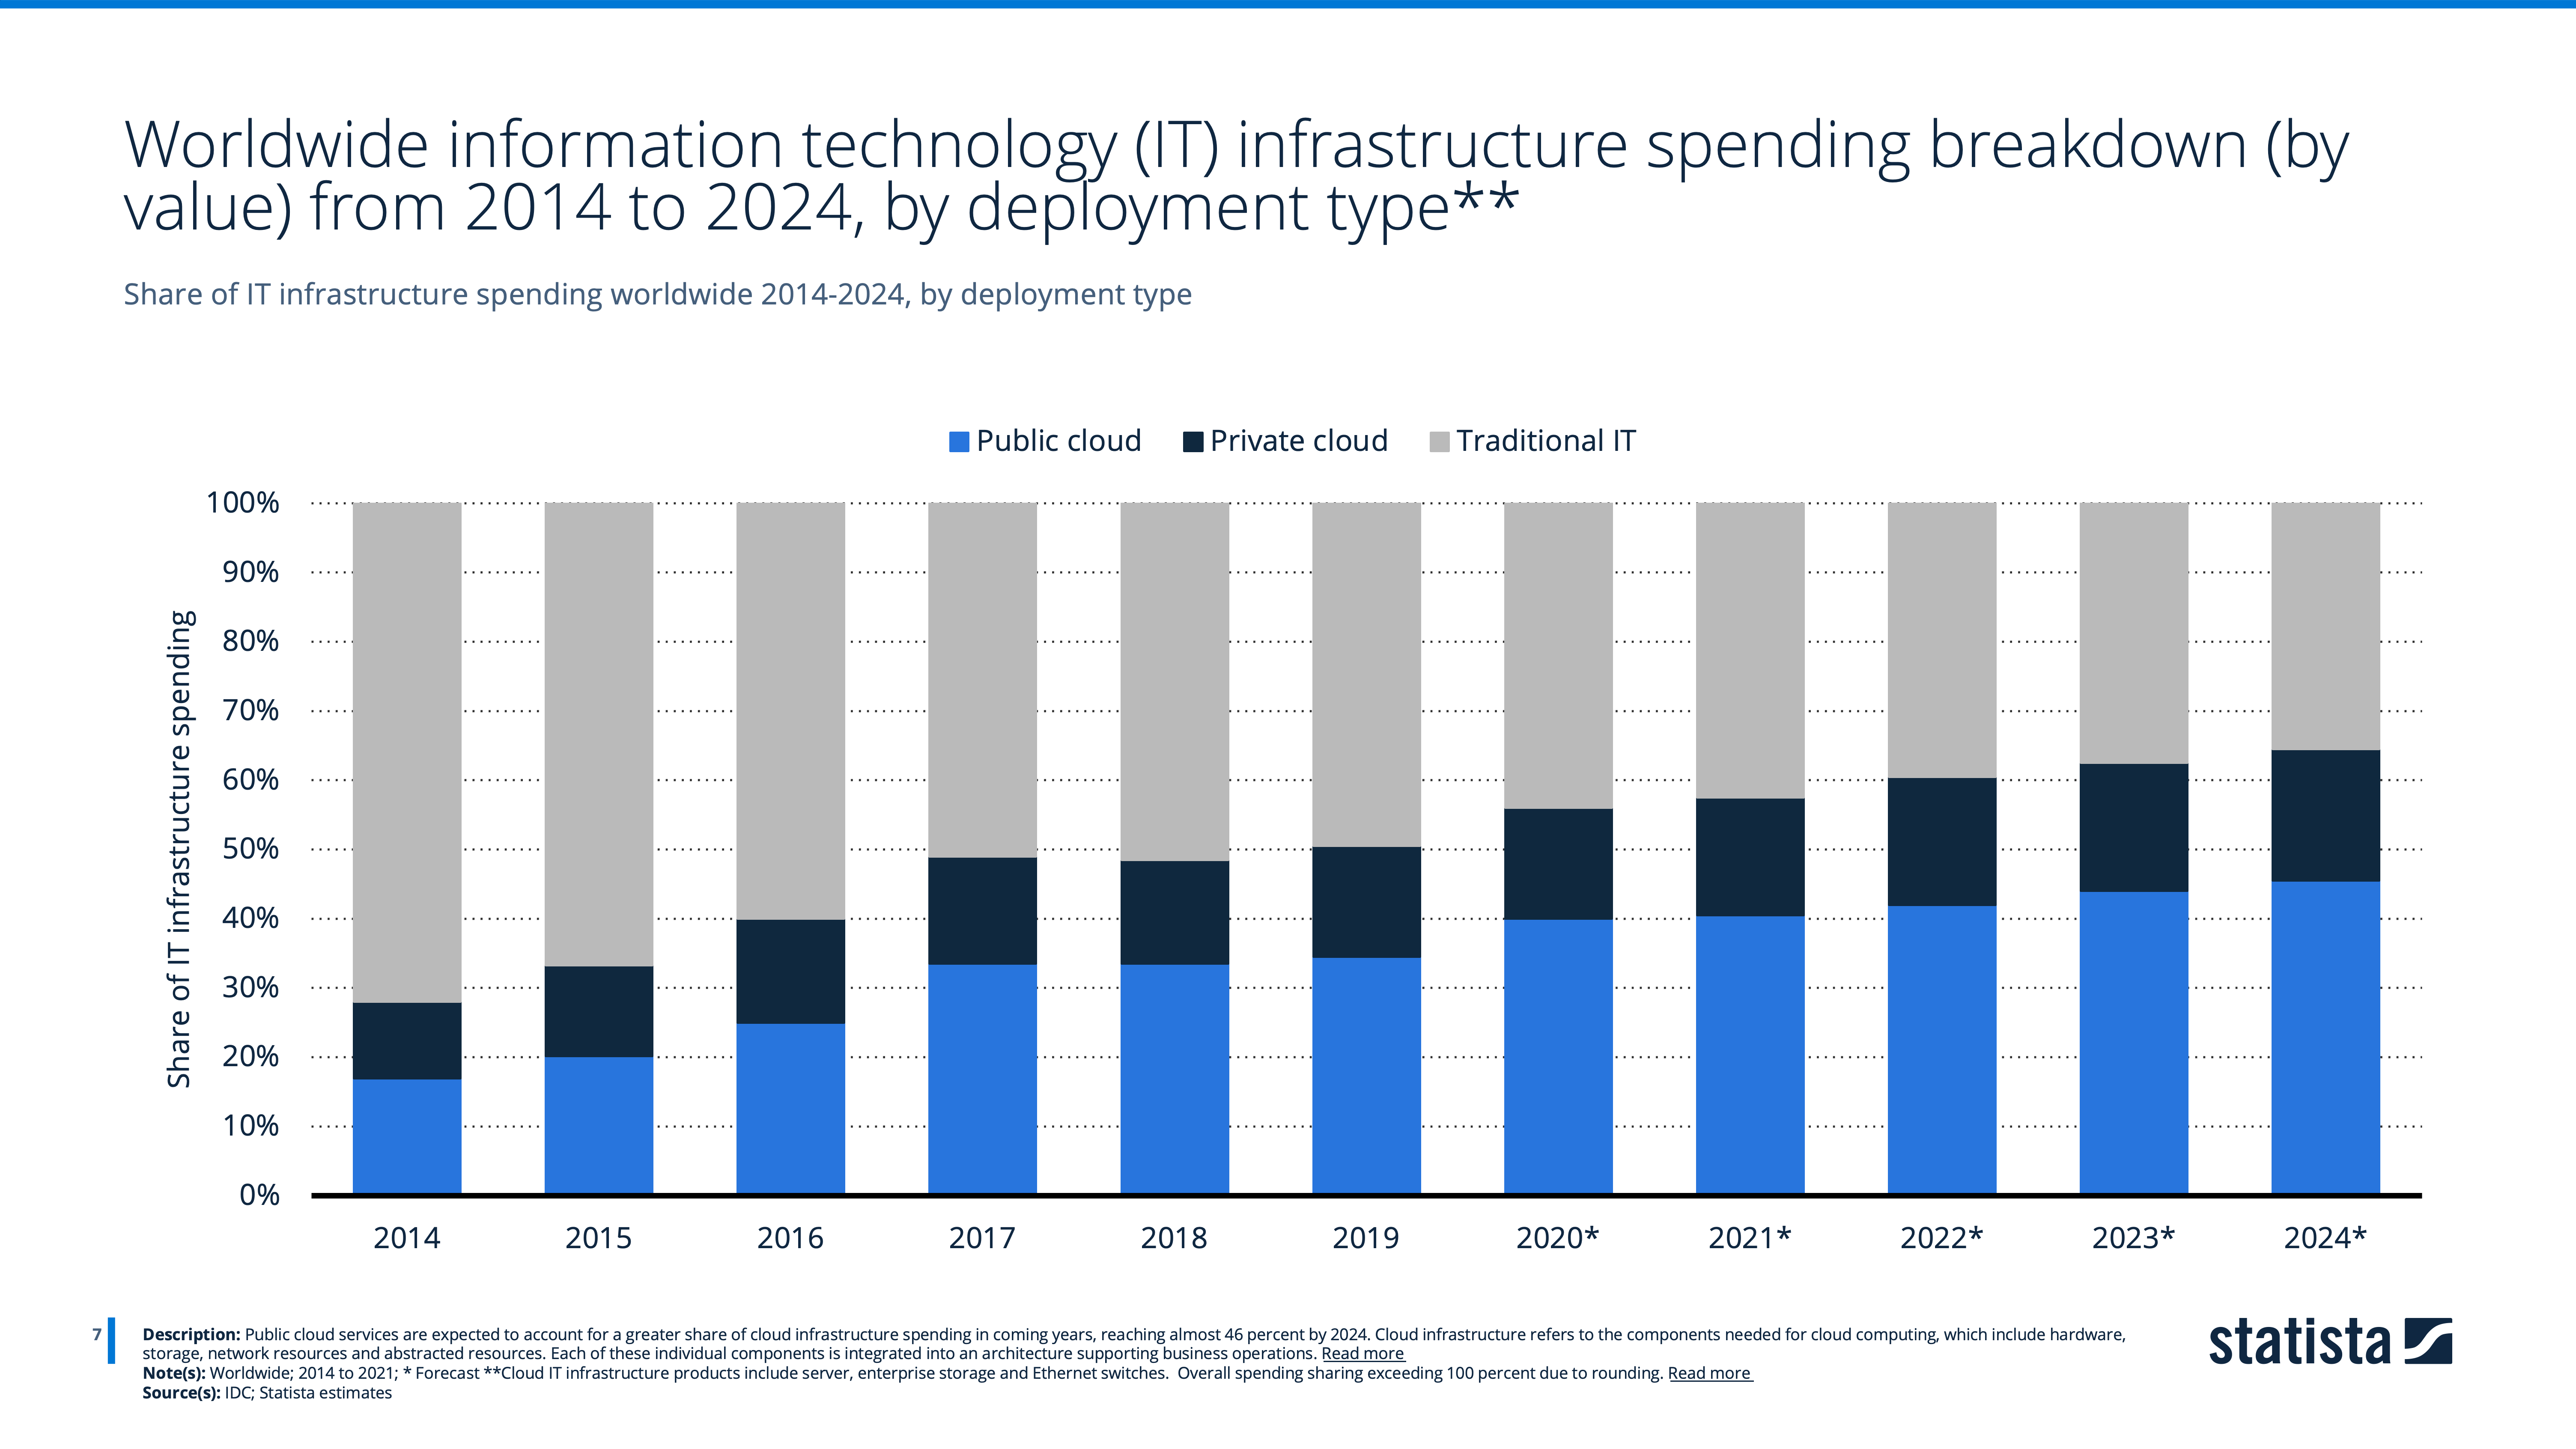
\includegraphics[width=\textwidth]{it_spending.png}
    \caption{Verteilung der Verkaufsleistungen für IT-Infrastruktur \cite[S. 7]{Statista2022}}
    \label{fig:it-spending}
\end{figure}

Daraus wird deutlich, wie Stark die Nutzung der Cloud, vorallem in den letzten Jahren, an Wert für Unternehmen gewonnen hat und dass sich diese Entwicklung fortsetzen wird.

Weitere Statistiken in dem Dossier zeigen, dass der Wachstum von Cloud Services seit 2018 bei konstant über 20\% liegt \cite[Vgl.][S. 6]{Statista2022} und Unternehmen jedes Jahr mehr Geld in die Nutzung von Public Cloud investieren \cite[Vgl.][S. 31f]{Statista2022}. \pagebreak

\subsection{Aktuelle Trends}
Im nachfolgenden Unterkapitel werden aktuelle Trends im Bereich des Cloud Computing anhand einiger Statistiken und Studien aufgezeigt, um einen Ausblick auf zukünftige Entwicklungen geben zu können.

\textbf{Wichtigkeit von Public Cloud}

\begin{figure}[H]
    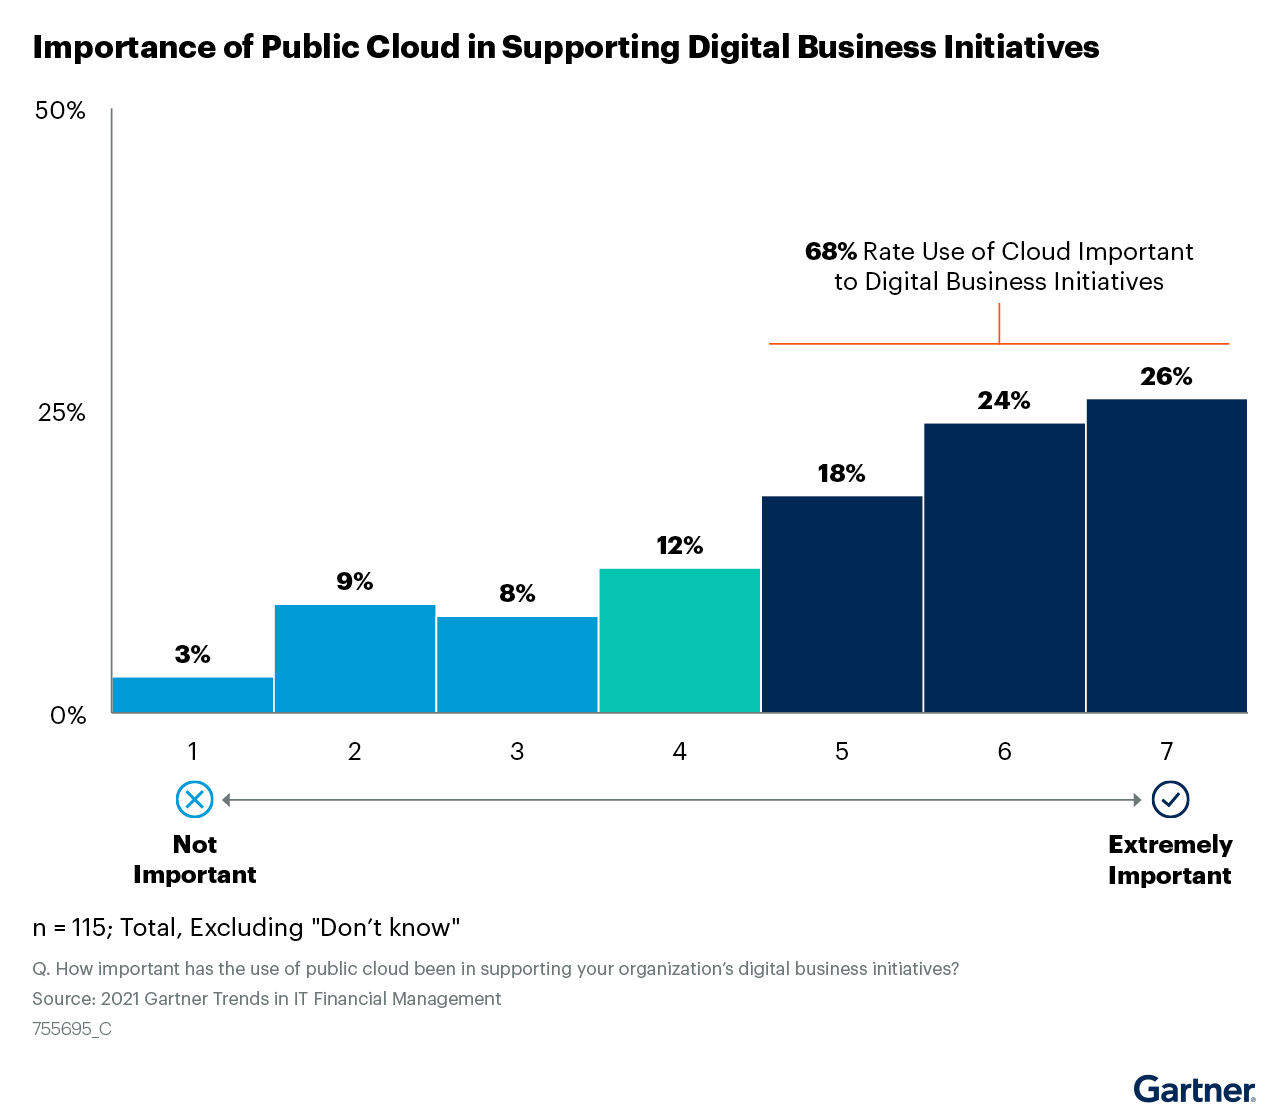
\includegraphics[width=\textwidth]{Figure_1_The_Importance_of_Public_Cloud_in_Supporting_Digital_Business_Initiatives.png}
    \caption{Bewertung der Wichtigkeit der Public Cloud \cite[S. 2]{Ganly2022}}
    \label{fig:importance}
\end{figure}

Abbildung \ref{fig:importance} zeigt aus einer Gartner Studie, welchen Stellenwert die Public Cloud bei den meisten Unternehmen hat. Knapp 70\% der Unternehmen haben hierbei einen Wert von über 5 angegeben (auf einer Skala von 1 bis 7), wobei sogar 26\% den höchsten Wert von 7 vergeben haben \cite[Vgl.][S. 2]{Ganly2022}. \pagebreak

\textbf{Cloud als nachhaltige Lösung}

Der Druck auf Unternehmen, Verantwortung für die Zukunft mit nachhaltigen Lösungen zu übernehmen, wächst stark. Unternehmen können durch die Nutzung der Cloud flexibler wählen welchen Provider diese nutzen wollen und darauf Achten, dass die Rechenzentren Klimaneutral betrieben werden \cite[Vgl.][S. 24ff]{Illsley2022}. \\

\textbf{Cloud-native Plattformen}

Eine weitere Gartner Studie von Chandrasekaran (2022) hat Cloud-Native Plattformen als einen der aktuellen strategischen Technologie Trends identifiziert und begründet diese Einordnung damit, dass moderne Anwendungsarchitekturen in Kombination mit der Cloud Technologie den Unternehmen neue Möglichkeiten verschaffen skalierbare Anwendungen zu entwickeln und damit die Digitalisierung vorantreiben \cite[Vgl][S. 12]{Chandrasekaran2022}. 

Um die Vorteile Cloud-nativer Anwendungen herauszuarbeiten, wird im nachfolgenden Kapitel detaillierter auf die Merkmale dieser eingegangen und wie sich damit die Vorteile des Cloud Computing besser ausnutzen lassen. \pagebreak